\section{Evaluación y resultados}
Una vez finalizada la fase de análisis cualitativo, se concluyó que el desarrollo de un sistema requiere de una arquitectura sólida sustentada en un paradigma adecuado, lo que garantiza organización del software. Asimismo, en el ámbito del agilismo, se evidenció la importancia de emplear una metodología debidamente estructurada, como Scrum, que permita adaptarse a los cambios, mejorar la comunicación entre los participantes del proyecto y facilitar la entrega incremental de funcionalidades. Estos hallazgos no solo orientaron las decisiones técnicas adoptadas en el proyecto formativo, sino que también aportaron criterios prácticos para optimizar la colaboración del equipo y la calidad del producto desarrollado. A partir de esto se obtuvieron resultados relevantes en tres planos:

\subsection{1. Resultados en la arquitectura y el desarrollo del sistema}
Se obtuvo un software basado en la arquitectura Modelo-Vista-Controlador (MVC), la cual permitió separar las responsabilidades en capas (modelo, vista y controlador), favoreciendo la organización del código. De manera complementaria, la adopción de la Programación Orientada a Objetos (POO) aportó principios como la reutilización, el encapsulamiento y la escalabilidad, lo que garantizó un desarrollo más estructurado y con mayor facilidad para la mantenibilidad y evolución futura del sistema.

\begin{figure}[htbp]
    \centering
    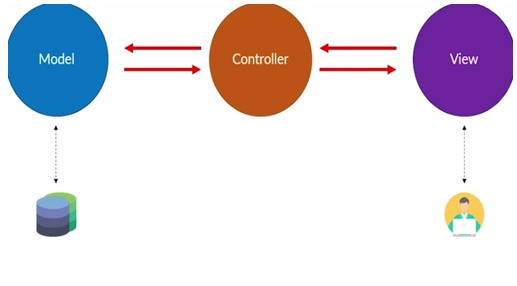
\includegraphics[width=0.8\textwidth]{graphics/mvc.jpeg}
    \caption{Modelo vista controlador}
    \label{fig:mvc}
\end{figure}

En la Figura \ref{fig:mvc} se ilustra la estructura de la arquitectura Modelo–Vista–Controlador (MVC) adoptada en el desarrollo del sistema de gestión de eventos. El uso de MVC permitió que cada componente pudiera desarrollarse y mantenerse de forma independiente, garantizando un código más organizado y facilitando la incorporación de nuevas funcionalidades sin afectar el resto del sistema.

\subsection{2. Resultados en la aplicación de la metodología ágil (Scrum)}
La implementación de la metodología ágil Scrum en el desarrollo del sistema generó beneficios tanto en el ámbito técnico como en el fortalecimiento de las habilidades blandas del equipo. En el plano técnico, permitió una adecuada planificación, control y seguimiento de los avances mediante la organización en sprints, lo que facilitó la adaptación a cambios y la entrega incremental de funcionalidades. En el plano humano, fomentó la comunicación constante, la colaboración y la responsabilidad compartida, promoviendo un ambiente de trabajo más dinámico y orientado a la resolución conjunta de problemas.

\begin{figure}[htbp]
    \centering
    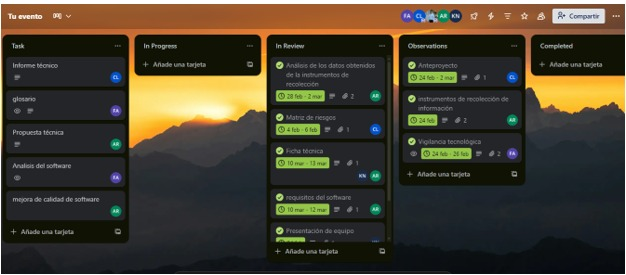
\includegraphics[width=0.8\textwidth]{graphics/trello.jpeg}
    \caption{Tablero trello}
    \label{fig:trello}
\end{figure}

En la Figura \ref{fig:trello} se observa el tablero de Trello empleado para la planificación y seguimiento de los sprints. Este recurso permitió visualizar las tareas pendientes, en progreso y completadas, facilitando la comunicación del equipo y el control de avances bajo la metodología ágil Scrum.